%!TEX root = generalexam.tex

% BEGIN CHAPTER

\cite{schwartz2010camresolution} demonstrated that quantitative precipitation forecasts benefit greatly from the use of high-resolution numerical models in both a deterministic and probabilistic framework. This is an important finding in that a majority of studies regarding cloud-resolving models used for producing forecast guidance more than a few hours in advance tend to be focused on deterministic results. It opens the door to such questions as, ``What should a storm-scale ensemble forecast system look like?'' It is becoming well established that convection-allowing models have shown improved skill in identifying regions where rare meteorological events associated with convection may occur -- especially when considered in the context of traditional numerical  models with parameterized convection. What has yet to be objectively demonstrated is how to best represent the uncertainty information from convection-allowing models.


Ensemble prediction systems have been a powerful tool in quantifying uncertainty in numerical forecasts; probabilistic forecast information is inherent in the ensemble generated output. For any given forecast field, one simply has to divide the number of numerical forecasts in which an event occurred divided by the number of numerical forecasts in which the event did not occur to receive a probability of an event occurring. One drawback to this method, however, is that probabilities generated are discrete, in intervals determined by the number of members in the ensemble. This poses significant challenges in how best to present traditional verification metrics such as reliability. One way to increase the resolution of the inherent probabilistic forecasts of ensemble prediction systems, one must increase the number of members, which, of course, requires additional computations resources or running numerical models at coarser grid spacing.


\cite{hamill1998eps} proposed a method for generating continuous probabilities from finite ensemble forecasts based on the ensemble's historical performance. This is best explained in an example. Consider a 4-member ensemble, where the sorted (highest-to-lowest) accumulated precipitation forecasts (in mm) are 40, 30, 20, and 10. To generate the probability that 25 mm or more of precipitation would accumulate, count the number of ensemble member's forecasts that exceed 25 mm and divide by the total number of ensemble members plus 1. Thus, $2 / (4+1) = 0.4$. However, that is the probability of exceeding 30 mm, no 25 mm; the probability of exceeding 25 mm should actually be greater than that of exceeding 30 mm. To account for this, determine the probability of exceeding the next lower ensemble threshold. Thus, $3 / (4+1) = 0.6$, yield a probability of exceedance of 60\%. The probability of exceeding 25 mm lies somewhere between 0.4 and 0.6. To determine the probability of exceeding 25 mm is determined by interpolating between the two values; the exact nature of this interpolation is determined by the ensemble's historical rank histogram.


The reason for using one more than the number of ensemble members in the divisor, instead of the number of ensemble members, becomes apparent when considering the two cases in which every ensemble member is either above or below the threshold at which one carries out the probability of exceedance. If every ensemble member produces precipitation, it is assumed that the probability of precipitation accumulating is unity. To put it another way, the probability of exceeding 0 mm is given a 100\% probability. If an ensemble member's forecast exceeds the forecast threshold (in the previous example it was 25 mm), the resulting (grid point) probability of exceedance is given by


$$
    POE = 1 - \left[\left(\frac{THRESH}{AMT_{min}}\right)(1 - PROB_{min})\right],
$$


\noindent where, $POE$ is the probability of exceeding the forecast threshold, given by $THRESH$, $AMT_{min}$ is the minimum forecast amount from any ensemble member (at the grid point), and $PROB_{min}$ is the probability of exceeding the amount forecast by the lowest ensemble member.


A similar exercise is undertaken for the case where every ensemble member forecasts amounts less than the threshold. In this case a linear extrapolation doesn't make sense. Considering again the example ensemble presented earlier, the probability of exceeding 50 mm should be greater than the probability of exceeding 100 mm. Thus, instead of a linear interpolation, a Gumbel distribution is used.


Unfortunately, as mentioned above, this method only makes use of forecasts at individual grid points. The very nature of a WoF paradigm is to produce forecasts of rare (in space and time) events. The intrinsic nature of rare events makes it unlikely that two separate high-resolution model forecasts would place identical phenomena at the same grid point, even for generally similar forecasts. Thus, creation and calibration of probabilistic forecasts of rare-events, such as those envisioned by WoF, requires a new approach.


This is a non-trivial task. Convection-allowing ensemble prediction systems are relatively new in the context of numerical modeling. Too little is known about the performance characteristics of convection-allowing models in explicitly predicting rare convective events, let alone understanding the performance of convection-allowing ensembles. This can be attributed to a number of reasons, chiefly among them is the relatively short duration of storm-scale ensemble forecast efforts \citep{done2004cams, clark2012overview} and poor observational datasets of rare convective hazards (e.g., \citealp{doswell1988stormreports, weiss2002stormreports, trapp2006stormreports, ortega2009shave}).


The composition of an ensemble's membership is an unsettled question in meteorological communities. Some believe that since initial condition errors tend to grow rapidly, that ensembles should consist solely of initial condition perturbations. Others argue that differences in model physics provide the most diversity of forecasts and thus ensembles should include some variations in physics packages. And still others argue that varying the model used produces the greatest impacts on at least features related to the land surface (surface temperature, moisture and winds -- all important in convective scale forecasts) is an important characteristic in an ensemble (\citealp{stensrud2000epscreation, eckel2005ensemble} and references contained within).  Ultimately, ensemble membership will most likely consist of combinations from all three viewpoints, but what remains to be seen what the optimal contributions from the various viewpoints will be.


There is a cost associated with adding a member to an ensemble. This cost is either computation, coming from either decreasing the horizontal and/or vertical grid spacing of every member, or monetary, stemming from the increased cost associated with additional computing and storage power. Thus a trade-off must be made when determining an ensemble's size. Arising out of this trade-off is the question, ``What is point of diminishing return with respect to ensemble size?'' In other words, at what point does the cost of adding additional members outweigh the contribution to forecast skill?


In some regards, these problems and questions have been the focus of an extraordinary collaborative effort between NSSL, SPC, and CAPS for several years through the Hazardous Weather Testbed Experimental Forecast Program (HWT-EFP). Although storm-scale models have been an important part of the HWT-EFP for a number of years, in 2011 CAPS was able to produce over 50, 4-km grid spacing numerical forecasts nightly. This has afforded HWT-EFP collaborators and participants an extraordinary opportunity to gain insights into how to create, transmit, visualize, and verify a storm-scale ensemble forecast system (SSEF). Additionally, this past year, Israel Jirak and Steve Weiss, both at SPC, championed the notion of a Storm-Scale Ensemble of Opportunity (SSEO) forecast system. The idea here was to take all the ``regularly'' available storm-scale forecasts and combine them together via post-processing techniques to produce probabilistic guidance of severe convective hazards.


What follows are thoughts on activities the HWT-EFP can undertake to examine these issues.




%%%%%%%%%%%%%%%%%%%%%%%%%%%%%
\section{Ensemble Membership}
%%%%%%%%%%%%%%%%%%%%%%%%%%%%%

The question of ensemble membership is difficult. The most obvious way to address this issue is to run various sets of ensembles and then examine the output. Fortunately, CAPS has been extremely successful in acquiring computational resources necessary to produce storm-scale ensemble forecasts. In 2010, CAPS produced a 15-member SSEF with grid spacing at 4 km, which grew to over 50 members in 2011. The 50 member SSEF of 2011 was comprised of several smaller ensembles including a 5 member ensemble, 15\footnote{The 15 member ensemble consisted of the same 15 members from 2010.} member ensemble, 18 member ensemble, and a 25\footnote{The 25th member was unavailable for a majority of the 2011 HWT-EFP.} member ensemble\footnote{The 5 member ensemble was a subset of the 15 member ensemble, which was a subset of the 25 member ensemble.} In the 25-member ensemble, 18 of the members were WRF-ARW cores, 5 were WRF-NMM (Nonhydrostatic Mesoscale Model) cores, and 1 was an Advanced Regional Prediction System (ARPS) Model. These models were initialized with a variations in initial and lateral boundary conditions and utilized different physics configurations. A list of the model configurations is given at the end of this chapter in Table \ref{ensemble_members}.


This unique dataset allows for simultaneous investigation into the questions previously presented.  The impacts of ensemble size can be explicitly evaluated from the perspective of 5, 15, and 25 members. The 18 member ensemble allowed for investigations into the impact of various choices for microphysics and planetary boundary layer (and combinations thereof), isolated from impacts of changing initial conditions. Granted a single HWT-EFP experiment, which consist of approximately 5 weeks of forecasts, is too small of a time-period (sample size) to draw vision altering results, however, it does allow one to frame the debate and develop questions for future investigations.




%%%%%%%%%%%%%%%%%%%%%
\section{Application}
%%%%%%%%%%%%%%%%%%%%%

The WoF vision of high-resolution, short-term forecasts of explicit severe convective hazards is still a long way from fruition on a CONUS scale, if for no other reason the National Oceanic and Atmospheric Administration's (NOAA) budget for both the National Weather Service and Office∫ of Ocean and Atmospheric Research does not allow for the necessary increases in computing power. In fact, the NWS National Centers for Environmental Prediction (NCEP) had to forgo its latest computing infrastructure upgrade and isn't scheduled for another one until 2014 (Weiss, personal communication 2011). However, much can be done in the interim.


Even though CONUS scale ensemble prediction systems capable of explicitly predicting convective hazards are many years off, convective scale ensembles, such as those run during the HWT-EFP, are certainly possible in the interim. One such real-time example of this is the High-Resolution Rapid Refresh (HRRR) model is now run hourly out to 15-hours \citep{smith2008hrrr}. Although a single deterministic model, research into the skill of time-lagged ensembles derived from models such as the HRRR should be evaluated. Along the same lines, a grass-roots type movement ensemble has been developed in-house at the SPC. At any given time there are approximately a half dozen or more storm-scale models that are valid. The ides behind the ``Storm-Scale Ensemble of Opportunity'' is that useful information can be gleaned from this ``opportunistic'' ensemble comprised of models provided by NSSL and NCEP's Environmental Modeling Center. Grass-roots approaches to furthering the WoF vision will continue to play a significant role over the next decade in answering the question of how to best apply storm-scale ensemble frameworks in operational settings.




%%%%%%%%%%%%%%%%%%%%%%
\section{Optimization}
%%%%%%%%%%%%%%%%%%%%%%

The question of ensemble optimization is rather open ended. What does it mean to optimize an ensemble anyways? Is determining ensemble membership part of the process of optimization? What about post-processing ensemble output? At least in the short term, the two are most likely related via the following question, ``What is the fewest number of members necessary to generate calibrated probabilistic forecasts when combined with statistical post-processing techniques?''  In a round about way, \cite{sobash2011kde} touched on this problem by utilizing kernel density estimation in a forecast sense. The method proposed by Sobash and coauthors took deterministic output and generated probabilistic fields. \cite{marsh2012callibration} expanded the kernel density estimation by developing a method to determine the the approximate smoothing values in an objective manner. Although this work was done in a deterministic framework, there are several methods in which it can be extended for using with ensembles. \cite{wilks2002smoothing} demonstrated that ensemble reliability can be improved by smoothing the output, which this method inherently does.


The benefit to approaches such as this will be computational savings by reducing the number of ensemble members necessary to capture the spread of possibilities and produce reliable forecasts. WoF will be computationally constrained for many years to come, so any method that can reduce the number of members necessary deserves further investigation.


Two drawbacks to statistical post processing techniques are the need for relatively large sample size of stable forecasts and high-resolution observations of the fields being forecast. The primary method to address the former problem is to simply wait long enough to create a sample of forecasts in which meaningful statistical techniques become appropriate. The latter method requires investment in methods of collecting high-resolution observations. Projects such as the Severe Hazards Analysis and Verification Experiment (SHAVE; \citealp{ortega2009shave}) and detailed surveys of high-impacts events, such as the damage surveys conducted of the 03 May 1999 tornado outbreak, are essential in establishing the observational datasets required for statistical post processing (not to mention, verification of forecasts).




%%%%%%%%%%%%%%%%%%%%%%%
\section{Visualization}
%%%%%%%%%%%%%%%%%%%%%%%

The issue of how to visualize information from high-resolution, storm-scale ensembles. Traditionally, forecasters are used to evaluating output from deterministic models. Forecasters can look, or at least give themselves the false sense of having looked, at everything there is to examine from a single model. As the WoF vision is realized, the flow of information will quickly make obsolete the option of examining all the model output. Instead methods of quickly visualizing \emph{and synthesizing} the output will be necessary. Recent HWT-EFPs have begun addressing this issue. Below is a sample of the work that has been started in this area, and it's potential benefits. It is a good start, but more work needs to be done.


\cite{marsh2010sls} utilized a web-display that allowed forecasters to choose various various smoothing parameters and view the resulting output from the 2010 HWT-EFP SSEF. Forecasters who preferred seeing detail in the probabilistic plots could choose smaller smoothing parameters and those who were comfortable with the larger smoothing parameters could choose those as well.  Additionally this web-display allowed forecasters to see the hourly probabilities of their choosing translate through space and time at hourly intervals, giving the forecaster a sense of how the ensemble as a whole evolved during that time frame.


In the 2011 HWT-EFP\footnote{Available at \url{http://hwt.nssl.noaa.gov/Spring_2011/ci_ens.php?date=20110524&p=6}.}, Marsh expanded the web-display to include many more options. Forecasters and researchers could choose to loop individual smoothed forecasts or the smoothed ensemble probabilities of various smoothing parameters. Since the ensemble was rather large, forecasters and researchers had an option to dynamically set the number of panels to display (typically in multiples of 3), and could choose what field to display in any of the windows. Additionally, forecasters and researchers could choose to turn on and off the option of displaying any of the individual members' forecasts of the phenomena in question. This allowed forecasters and researchers to visualize how phenomena from individual members contributed to the probabilities for that member. Additionally, forecasters and researchers to be able to overlay the specific phenomena from any member on the background probability of the ensemble. Feedback from participants suggests that web-displays of this sort are absolutely crucial for people evaluating ensembles to be able to interrogate the data while keeping a sense of the probabilistic information offered by the ensemble.


Additional displays are either in the works or need to be created. Marsh has committed to creating the capability display forecast soundings from ensembles in a manner that is convenient to compare them to observations from both traditional (radiosondes) and non-traditional sources (radiometers, Doppler LIDARs, etc) on time scales of the observing platforms. In other words, being able to display model soundings at 5 minute intervals in comparison to a radiometer. Tools like this should allow for researchers to quickly visualize and synthesize how a model predicted boundary layer is evolving compared to those observed.


Additional effort should be given toward means of extracting statistical information from individual members as well as the entire ensemble in a efficient and dynamical manner.




%%%%%%%%%%%%%%%%%%%%%%
\section{Verification}
%%%%%%%%%%%%%%%%%%%%%%

Any discussion about convective ensembles and the WoF initiative would be remiss if it didn't include discussion regarding verification. As numerical models continue to run at finer and finer grid spacing, it becomes harder and harder to measure improvements in the models' performances. Verification metrics ultimately depend on what it is one cares about. If someone cares about improving forecast skill, a different norm might be chosen than someone who cares about improving model dynamics \citep{hacker2005predictability}. Since WoF has an explicit goal related to prediction of high-impact convective hazards, this discussion will focus on the problem of improving forecast skill.


As briefly touched upon earlier in this chapter, a major component surrounding the issue of improving forecast skill is that as the number of grid points contained within a model increase, the number of grid points available for a model to resolve it's solution increases. Traditional verification metrics penalize high-resolution models for displacement errors, even if the high-resolution model conveyed the general idea of the forecast. For example, traditional verification metrics would tend to lead users in believing a model had very poor skill if the model was off on its forecast by one grid space everywhere, even though human forecasters would most likely consider it a successful forecast. As noted in \cite{clark2009comparison}, and discussed yearly among HWT-EFP collaborators, better verification metrics must be explored, and object-based metrics are a leading candidate.


Another problem regarding the measuring of forecast skill is that producing the most skillful forecasts (such as in terms of reliability) might not provide the most useful information to forecasters. Take for example the work by \cite{marsh2012calibration}. Marsh and coauthors have developed a method to generate probabilistic forecasts of rare events from deterministic forecasts that are more statistically reliable than the 2011 HWT-EFP 25 member SSEF (Figs. \ref{fig:nssl}, \ref{fig:ssef}, and \ref{fig:roc rely}). However subjective impressions of the resulting output is that the probability field is ``too smooth''. During the 2011 HWT-EFP most visiting forecasters did not use the product in the course of their forecast process.  Forecasters have a tendency to want to look at fields that do not smooth out the underlying signal and thus prefer looking at fields with less smoothing, even if it the resulting probabilistic fields are not reliable. Verification metrics that adequately capture the subconscious metrics used by human forecasters are sorely needed.


Lastly, as ensemble simulations, such as the HRRR and, in particular, those produced by CAPS, become more common, \cite{hamill2006trueskill} offer a warning of sorts regarding understanding model skill. Model skill must be understood in the context of the climatological event frequency, especially across vast spatial domains. Is a model's perceived skill the result of actual skill or spatially varying climatological frequencies? In particular, \cite{hamill2006trueskill} urge caution when using the Brier Skill Score, Relative Operating Characteristics, and Equitable Threat Scores. In particular, caution is implored when positive skill is diagnosed from reference climatological forecasts when distinct climatologies can be identified in subsets of the parent dataset. This perceived skill may actually be the result of underlying differences in the various distinct climatologies represented by a single climatological norm.


To address these potential issues, verification should be carried out over each of regions that have distinct climatologies. Alternatively, consider computing skill scores from each distinct climatology using local climatological distributions, such as exceeding various quantiles. This implicitly accounts for varying means and variances across the different climatologies and ensures that the same fraction of data are used. Ultimately, whatever metric is used, the specific details should be fully disclosed for reproducibility.




%%%%%%%%%%%%%%%%%%%%%%%%%%%
%!TEX root = prospectus.tex


% ENSEMBLE DATA



%%%%%%%%%%%%%%%%%%%%%%%%%%%%%%%%%%%%%%%%%%%%%%%%%
%%%                                           %%%
%%%                  TABLES                   %%%
%%%                                           %%%
%%%%%%%%%%%%%%%%%%%%%%%%%%%%%%%%%%%%%%%%%%%%%%%%%

\newpage

\begin{center}
    \renewcommand{\arraystretch}{3}
    \centering
    \singlespace
    \rowcolors{2}{gray!20}{white}
    \begin{longtable}{|c|c|c|c|c|c|c|}
        \caption[Configurations for the 2011 CAPS Ensemble Members]
        {Configurations for the 2010 and 2011 CAPS Ensemble Members. Members listed in red are those used in both 2010 and 2011.}
        \label{ensemble_members} \\

        % Header for the first page
        \hline
        \rowcolor{gray!60}
        \member{\textbf{Member}} &
        \ic{\textbf{Initial Conditions}} &
        \bc{\textbf{Boundary Conditions}} &
        \radar{\textbf{Radar Data}} &
        \microphysics{\textbf{Microphysics}} &
        \lsm{\textbf{LSM}} &
        \pbl{\textbf{PBL}} \\
        \hline
        \endfirsthead

        % Header for remaining pages
        \multicolumn{7}{c}{{\tablename} \thetable{} -- Continued} \\
        \hline
        \rowcolor{gray!60}
        \member{\textbf{Member}} &
        \ic{\textbf{Initial Conditions}} &
        \bc{\textbf{Boundary Conditions}} &
        \radar{\textbf{Radar Data}} &
        \microphysics{\textbf{Microphysics}} &
        \lsm{\textbf{LSM}} &
        \pbl{\textbf{PBL}} \\
        \hline
        \endhead

        %This is the footer for all pages except the last page of the table...
        \multicolumn{7}{l}{{Continued on Next Page \ldots}} \\
        \endfoot

        %This is the footer for the last page of the table...
        \hline \hline
        \multicolumn{7}{l}{Note 1: For all members, \emph{cu\_physics} = None} \\
        \multicolumn{7}{l}{Note 2: For all ARW members, \emph{ra\_lw\_physics} = RRTM} \\
        \multicolumn{7}{l}{Note 3: For all ARW members, \emph{ra\_sw\_physics} = Goddard} \\
        \multicolumn{7}{l}{Note 4: For nmm\_cn, nmm\_m2, \& nmm\_m3, \emph{ra\_lw\_physics} = GFDL;
            \emph{ra\_sw\_physics} = GFDL} \\
        \multicolumn{7}{l}{Note 5: For nmm\_m4 \& nmm\_m5, \emph{ra\_lw\_physics} = RRTM;
            \emph{ra\_sw\_physics} = Dudhia} \\
        \multicolumn{7}{l}{Note 6: The arps member uses Chou/Suarex for radiation.} \\
        \multicolumn{7}{l}{Note 7: Ferrier+ refers to a subset of changes in the updated
            version now in NEMS/NMMB.} \\

        \endlastfoot

        % Member 1 of 24
        \hline
        \coremem\member{arw\_cn} &
        \coremem\ic{00Z ARPS 3DVAR \& Cloud Analysis} &
        \coremem\bc{00Z NAM Forecast} &
        \coremem\radar{Yes} &
        \coremem\microphysics{Thompson} &
        \coremem\lsm{Noah} &
        \coremem\pbl{MYJ} \\

        % Member 2 of 24
        \hline
        \coremem\member{arw\_m4} &
        \coremem\ic{arw\_cn + em\_p1\_pert} &
        \coremem\bc{21Z SREF em\_p1} &
        \coremem\radar{Yes} &
        \coremem\microphysics{Morrison} &
        \coremem\lsm{RUC} &
        \coremem\pbl{YSU} \\

        % Member 3 of 24
        \hline
        \coremem\member{arw\_m5} &
        \coremem\ic{arw\_cn + em\_p2\_pert} &
        \coremem\bc{21Z SREF em\_p2} &
        \coremem\radar{Yes} &
        \coremem\microphysics{Thompson} &
        \coremem\lsm{Noah} &
        \coremem\pbl{QNSE} \\

        % Member 4 of 24
        \hline
        \coremem\member{arw\_m6} &
        \coremem\ic{arw\_cn - nmm\_p1\_pert} &
        \coremem\bc{21 SREF nmm\_p1} &
        \coremem\radar{Yes} &
        \coremem\microphysics{WSM6} &
        \coremem\lsm{RUC} &
        \coremem\pbl{QNSE} \\

        % Member 5 of 24
        \hline
        \coremem\member{arw\_m7} &
        \coremem\ic{arw\_cn + nmm\_p2\_pert} &
        \coremem\bc{21Z SREF nm\_p2} &
        \coremem\radar{Yes} &
        \coremem\microphysics{WDM6} &
        \coremem\lsm{Noah} &
        \coremem\pbl{MYNN} \\

        % Member 6 of 24
        \hline
        \coremem\member{arw\_m8} &
        \coremem\ic{arw\_cn + rsm\_n1\_pert} &
        \coremem\bc{21Z SREF rsm\_n1} &
        \coremem\radar{Yes} &
        \coremem\microphysics{Ferrier} &
        \coremem\lsm{RUC} &
        \coremem\pbl{YSU} \\

        % Member 7 of 24
        \hline
        \coremem\member{arw\_m9} &
        \coremem\ic{arw\_cn - etaKF\_n1\_pert} &
        \coremem\bc{21Z SREF etaKF\_n1} &
        \coremem\radar{Yes} &
        \coremem\microphysics{Ferrier} &
        \coremem\lsm{Noah} &
        \coremem\pbl{YSU} \\

        % Member 8 or 24
        \hline
        \coremem\member{arw\_m10} &
        \coremem\ic{arw\_cn + etaKF\_p1\_pert} &
        \coremem\bc{21Z SREF etaKF\_p1} &
        \coremem\radar{Yes} &
        \coremem\microphysics{WDM6} &
        \coremem\lsm{Noah} &
        \coremem\pbl{QNSE} \\

        % Member 9 of 24
        \hline
        \coremem\member{arw\_m11} &
        \coremem\ic{arw\_cn - etaBMJ\_p1\_pert} &
        \coremem\bc{21Z SREF etaBMJ\_p1 } &
        \coremem\radar{Yes} &
        \coremem\microphysics{WSM6} &
        \coremem\lsm{RUC} &
        \coremem\pbl{MYNN} \\

        % Member 10 of 24
        \hline
        \coremem\member{arw\_m12} &
        \coremem\ic{arw\_cn + etaBMJ\_p1\_pert} &
        \coremem\bc{21Z SREF etaBMJ\_p1} &
        \coremem\radar{Yes} &
        \coremem\microphysics{Thompson} &
        \coremem\lsm{RUC} &
        \coremem\pbl{MYNN} \\

        % Member 11 of 24
        \hline
        \member{arw\_m13} &
        \ic{arw\_cn + rsm\_p1\_pert} &
        \bc{21Z SREF rsm\_p1} &
        \radar{Yes} &
        \microphysics{M-Y} &
        \lsm{Noah} &
        \pbl{MYJ} \\

        % Member 12 of 24
        \hline
        \member{arw\_m14} &
        \ic{arw\_cn + em\_n1\_pert} &
        \bc{21 SREF em\_n1} &
        \radar{Yes} &
        \microphysics{Ferrier+} &
        \lsm{Noah} &
        \pbl{YSU} \\

        % Member 13 of 24
        \hline
        \member{arw\_m15} &
        \ic{arw\_cn + em\_n2\_pert} &
        \bc{21Z SREF em\_n2} &
        \radar{Yes} &
        \microphysics{WSM6} &
        \lsm{Noah} &
        \pbl{MYNN} \\

        % Member 14 of 24
        \hline
        \member{arw\_m16} &
        \ic{arw\_cn + nmm\_n1\_pert} &
        \bc{21Z SREF nmm\_n1} &
        \radar{Yes} &
        \microphysics{Ferrier+} &
        \lsm{Noah} &
        \pbl{QNSE} \\

        % Member 15 of 24
        \hline
        \member{arw\_m17} &
        \ic{arw\_cn + nmm\_n2\_pert} &
        \bc{21Z SREF nmm\_n2} &
        \radar{Yes} &
        \microphysics{Thompson} &
        \lsm{Noah} &
        \pbl{ACM2} \\

        % Member 16 or 24
        \hline
        \member{arw\_m18} &
        \ic{arw\_cn + rsm\_p2\_pert} &
        \bc{21Z SREF rsm\_p2} &
        \radar{Yes} &
        \microphysics{WSM6} &
        \lsm{Noah} &
        \pbl{MYJ} \\

        % Member 17 of 24
        \hline
        \member{arw\_m19} &
        \ic{arw\_cn + rsm\_n1\_pert} &
        \bc{21Z SREF rsm\_n1} &
        \radar{Yes} &
        \microphysics{M-Y} &
        \lsm{Noah} &
        \pbl{MYJ} \\

        % Member 18 of 24
        \hline
        \member{arw\_m20} &
        \ic{arw\_cn + rsm\_n2\_pert} &
        \bc{21Z SREF rsm\_n2} &
        \radar{Yes} &
        \microphysics{M-Y} &
        \lsm{RUC} &
        \pbl{ACM2} \\

        % Member 19 of 24
        \hline
        \coremem\member{nmm\_cn} &
        \coremem\ic{00Z ARPS 3DVAR \& Cloud Analysis} &
        \coremem\bc{00Z NAM Forecast} &
        \coremem\radar{Yes} &
        \coremem\microphysics{Ferrier} &
        \coremem\lsm{Noah} &
        \coremem\pbl{MYJ} \\

        % Member 20 of 24
        \hline
        \member{nmm\_m2} &
        \ic{nmm\_cn + em\_n2\_pert} &
        \bc{21 SREF em\_n2} &
        \radar{Yes} &
        \microphysics{Ferrier+} &
        \lsm{Noah} &
        \pbl{MYJ} \\

        % Member 21 of 24
        \hline
        \coremem\member{nmm\_m3} &
        \coremem\ic{nmm\_cn + nmm\_n1\_pert} &
        \coremem\bc{21Z SREF nmm\_n1} &
        \coremem\radar{Yes} &
        \coremem\microphysics{Thompson} &
        \coremem\lsm{Noah} &
        \coremem\pbl{MYJ} \\

        % Member 22 of 24
        \hline
        \coremem\member{nmm\_m4} &
        \coremem\ic{arw\_cn + nmm\_n2\_pert} &
        \coremem\bc{21Z SREF nmm\_n2} &
        \coremem\radar{Yes} &
        \coremem\microphysics{WSM6} &
        \coremem\lsm{RUC} &
        \coremem\pbl{MYJ} \\

        % Member 23 of 24
        \hline
        \coremem\member{nmm\_m5} &
        \coremem\ic{arw\_cn + em\_n1\_pert} &
        \coremem\bc{21Z SREF em\_n1} &
        \coremem\radar{Yes} &
        \coremem\microphysics{Ferrier} &
        \coremem\lsm{RUC} &
        \coremem\pbl{MYJ} \\

        % Member 24 or 24
        \hline
        \coremem\member{arps\_cn} &
        \coremem\ic{00Z ARPS 3DVAR \& Cloud Analysis} &
        \coremem\bc{00Z NAM Forecast} &
        \coremem\radar{Yes} &
        \coremem\microphysics{Lin} &
        \coremem\lsm{Force Restore} &
        \coremem\pbl{??? ???} \\
        \hline

    \end{longtable}
\end{center}




\label{2011ssef}
%%%%%%%%%%%%%%%%%%%%%%%%%%%




%%%%%%%%%%%%%%%%%%%%%%%%%%%%%%%%%%%%%%%%%%%%%%%%%
%%%%%%%%%%           FIGURES           %%%%%%%%%%
%%%%%%%%%%%%%%%%%%%%%%%%%%%%%%%%%%%%%%%%%%%%%%%%%

\newpage


\begin{figure}
    \begin{center}
        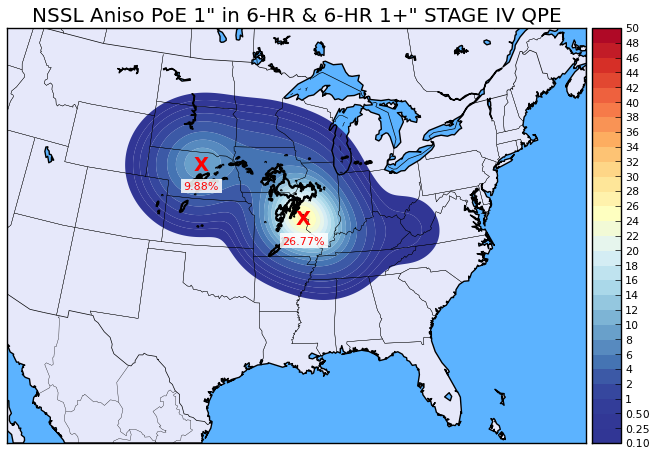
\includegraphics[scale=0.50]{figs/nssl.png}
        \caption{\small Sample probabilistic post-processed output generated from the NSSLWRF using the method put forth by \cite{marsh2012calibration}. The forecast threshold is 25.4 mm in 6 h.}
        \label{fig:nssl}
    \end{center}
\end{figure}


\begin{figure}
    \begin{center}
        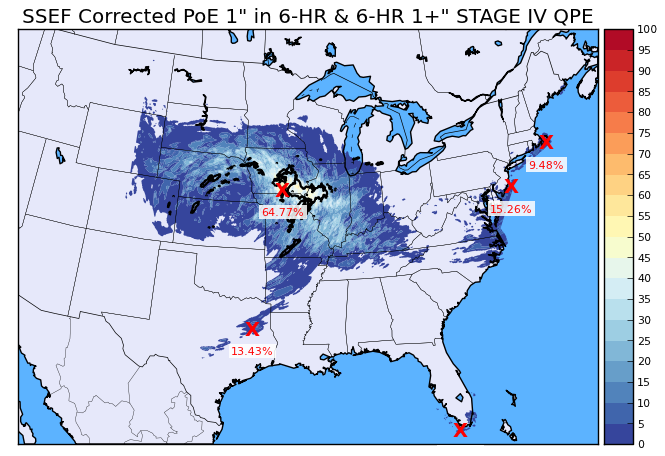
\includegraphics[scale=0.50]{figs/ssef.png}
        \caption{\small Sample probabilistic post-processed output created from the HWT-EFP 2011 25 member storm-scale ensemble forecast system. The probabilisties here were generated using the method put forth by \cite{hamill1998eps}. The forecast threshold is 25.4 mm in 6 h, and is valid for the same time period as in Fig. \ref{fig:nssl}.}
        \label{fig:ssef}
    \end{center}
\end{figure}


\begin{figure}
    \begin{center}
        \includegraphics[scale=0.4]{figs/roc_rely.pdf}
        \caption{\small The ROC curve and reliability diagram comparing probabilistic output from the NSSLWRF using the methods of \cite{marsh2012calibration} as compared to the output generated from the 2011 HWT-EFP 25 member SSEF. Forecasts were only evaluated over time periods where both the SSEF and NSSLWRF were available.}
        \label{fig:roc rely}
    \end{center}
\end{figure}